\section{Renormalization Group Procedure for Effective Particles (RGPEP)}
\label{sec:rgpep}

Divergences appering in Hamiltonian quantum field theories come from far off-diagonal matrix elements. 
These matrix elements arise from interactions between particles of vastly different energy scales. 
For example, consider the following interaction present in Yukawa theory, $fb \rightarrow f$:
\begin{figure}[h]
    \label{fig:interaction}
    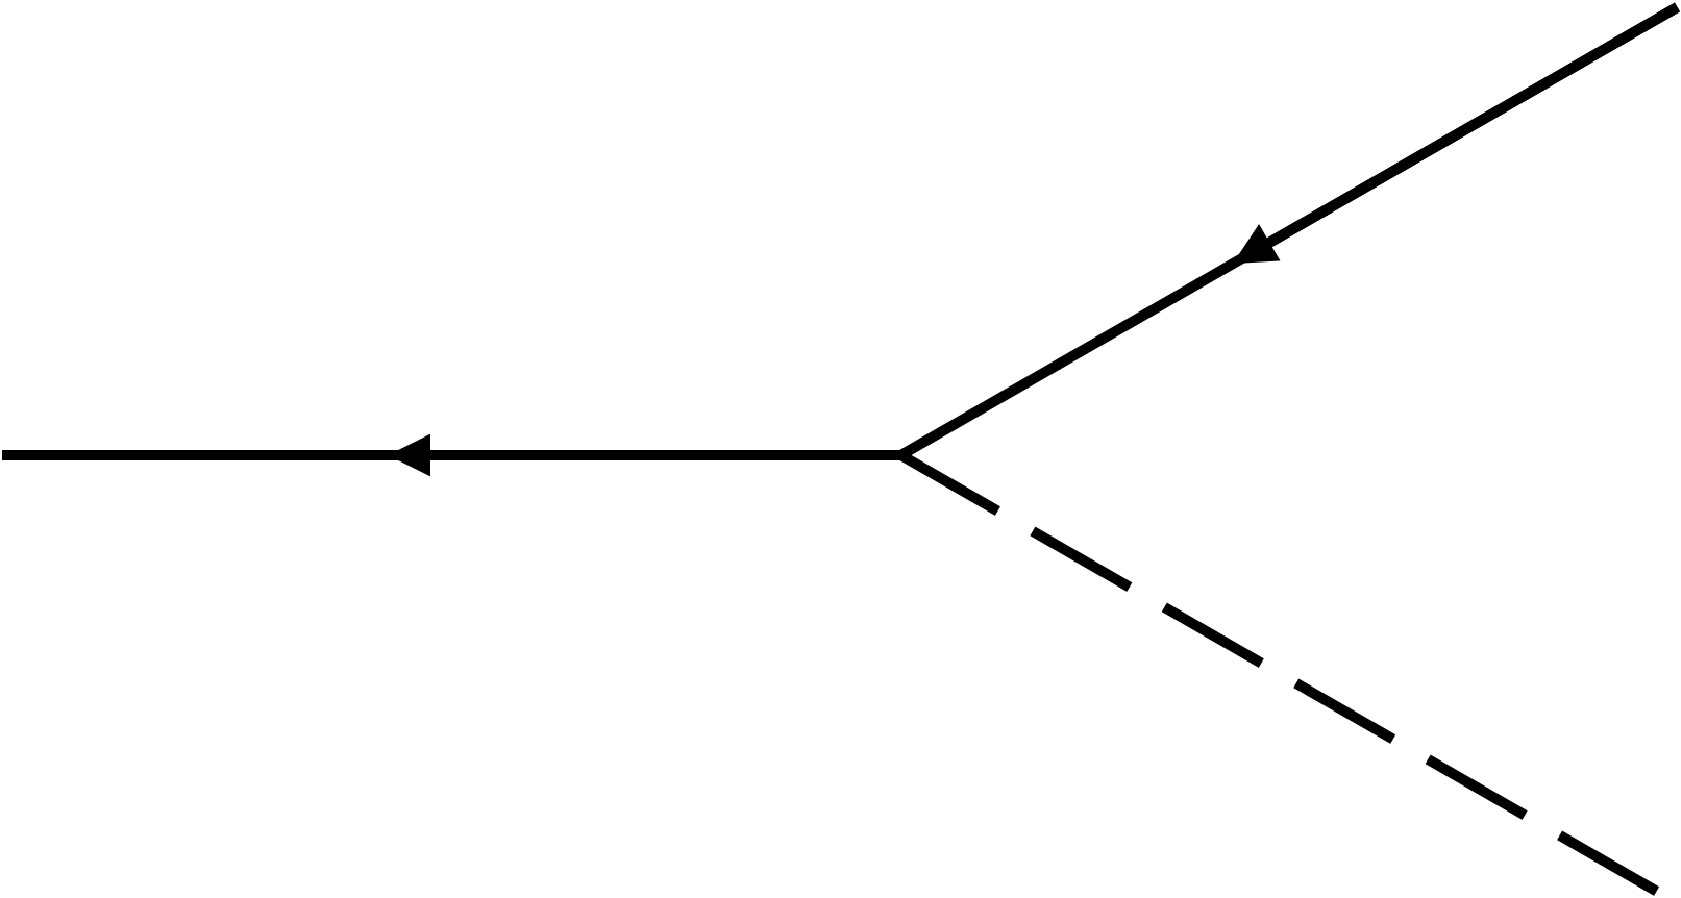
\includegraphics[width = 0.5\textwidth, height = 0.25\textwidth]{figures/interaction.pdf}
    \caption{Interaction}
\end{figure}

